\subsection{Capturing syntactic dependencies}
\label{sec:dependencies}

Words encapsulate linguistic information into units that are then put
into relation by syntactic rules. A long tradition in linguistics has
even claimed that syntax is blind to sub-word-level processes
\cite[e.g.,][]{Chomsky:1970,DiSciullo:Williams:1987,Bresnan:Mchombo:1995,Williams:2007}. Can
our CNLMs, despite the lack of an explicit word lexicon, capture
relational syntactic phenomena, such as agreement and case assignment?
We investigate this by testing them on syntactic dependencies between
non-adjacent words. We adopt the ``grammaticality judgment'' paradigm
of \newcite{Linzen:etal:2016}. We create minimal sets of grammatical
and ungrammatical phrases illustrating the phenomenon of interest, and
let the language model assign a likelihood to all items in the
set. The language model is said to ``prefer'' the grammatical variant
if it assigns a higher likelihood to it than to its ungrammatical
counterparts. We must stress two methodological points. First, since a
character-level language model assigns a probability to each character
of a phrase, and the phrase likelihood is the product of these values
(all between 0 and 1), minimal sets must be controlled for character
length. This makes existing benchmarks unusable. Second, the
``distance'' of a relation is defined differently for a
character-level model, and it is not straightforward to
quantify. Consider the German phrase in \ref{ex:german-gender}
below. For a word model, two items separate the article from the
noun. For a (space-less) character model, 8 characters intervene until
the noun onset, but the span to consider will typically be longer. For
example, \emph{Baum} could be the beginning of the feminine noun
\emph{Baumwolle} ``cotton'', which would change the agreement
requirements on the article. So, until the model finds evidence that
it fully parsed the head noun, it cannot reliably check
agreement. This will typically require parsing at least the full noun
and the first character following it. We again focus on German and Italian, as their richer inflectional
morphology simplifies the task of constructing balanced minimal sets.


%\textbf{Please provide size for all evaluation sets.}

%\textbf{In the interest of space, please reduce figures ~\ref{fig:gender}, ~\ref{fig:case} and \ref{fig:prep} to a single figure with 3 panels: the averaged gender and case results, and the subcategorization case. Also, either put titles on the figures, or at least label them as a), b) c). Legends should be LSTM, RNN and WordNLM (or WNLM) for coherence.}XS

%We take a further step up the linguistic hierarchy, probing CNLMs for their ability to capture syntactic dependencies between non-adjacent words. %
% --a rather challenging task for models that work entirely at the character level, and do not even have information about what words are.
% % Despite not having predefined information about words and
% % morphemes, is the model able to capture non-adjacent syntactic
% % dependencies?
% In particular, is it able to do so when dependencies cross one or more words, and thus cannot be reduced to surface n-gram counts?
% Note that, for a CNLM, dependencies across even a single word are often already long-distance. % even \emph{``\textbf{la} bell\textbf{a}''} is long distance.
% We again focus on German and Italian due to the richness of inflectional morphology in these languages.
% Constructions will be language-specific, so we discuss the languages separately. %German and Italian separately (not much in English).

%As usual, specifics of training etc that depart from general setup.

\subsubsection{German}%  We consider 4 constructions:
% \begin{inparaenum}[i)]
% \item article-noun gender agreement, possibly with material in the middle,
% \item determiner-noun case concord, again with material in the middle,
% \item preposition case sub-categorization, with material in the middle.
% \end{inparaenum}


\paragraph{Gender agreement}
Each German noun belongs to one of three genders (masculine, feminine, neuter), morphologically marked on the article. As the article and the noun can be separated by adjectives and adverbs, we can probe knowledge of nouns' lexical gender together with long-distance agreement.
We create stimuli of the form
\exg. \{\underline{der},\ die,\ das\} sehr rote Baum \\
the very red tree \\
%    article adverb adjective noun\\
%    `the very red tree'

%\begin{enumerate}[label={(\arabic*)}]
%	\item \begin{tabular}[t]{lllllll}
%	\{\underline{der}, die, das\}& sehr& rote& Baum \\
%	article & adverb & adjective & noun \\
%	the & very & red & tree
%\end{tabular}
%\end{enumerate}
where the correct nominative singular article (\emph{der}, in this case) matches the gender of the noun.
We then run the CNLM on the three versions of this phrase (removing whitespace) and record the probabilities it assigns to them. If the model assigns the highest probability to the version with the right article, we count it as a hit for the model. To avoid phrase segmentation ambiguities, we present phrases surrounded by full stops.

%  \cite{de2006generating,mcdonald2013universal}
We select all nominative singular nouns from the German UD treebank. %, and all adjectives from the training set.
We construct four conditions varying the number of adverbs and adjectives between  article and noun.
We first consider stimuli where no material intervenes. % \footnote{Due to syncretism in the article paradigm, there is sometimes ambiguity in the choice of the correct article if the noun's morphology does not uniquely indicate that it is a nominative singular from. As this equally affects all feminine nouns, we did not remove such cases. Importantly, this issue is solved as soon as an adjective intervenes, as its form disambiguates case.}
In the second condition, an adjective with the correct (nominative singular) case ending, randomly selected from the training corpus, is added. Crucially, the ending of the adjective does not reveal the gender of the noun.
In the third and fourth conditions, one (\emph{sehr}) or two adverbs (\emph{sehr extrem}) intervene between the article and the adjective. These do not cue gender either. In each condition, we obtained 2290 (m.), 2261 (f.), and 1111 (n.) stimuli.

We constructed an n-gram baseline that picks the article occurring
most frequently before the phrase in the training data, choosing
randomly in case of ties. Here and below, when running the
WordNLM, we excluded OOV nouns, resulting in a slightly easier test
for this rival model. However, testing the CNLMs on the reduced set
only led to slight improvements, that we do not report here.

Results are presented in Figure~\ref{fig:german-syntax}
(left). WordNLM performs best, followed by the LSTM CNLM.  While the
n-gram baseline performs similarly to the CNLM when there is no
intervening material, accuracy drops to chance level (0.33) in the
presence of an adjective. This problem would not be mitigated by
interpolation with or backoff to lower-order n-grams, as the relevant
gender information is present only on the first and last word of each
stimulus. We conclude that, while direct association between articles
and nouns can be learnt from simple corpus statistics, the CNLM has
some capability to preserve the relevant information across more than
a dozen timesteps. The RNN CNLM is much worse than the LSTM
counterpart and even the n-gram model for the adjacent context, and
its accuracy drops to random as more material intervenes, further
confirming the importance of storing long-distance information. Note
that, at the character level, even ``adjacent'' agreement requires
carrying information through multiple time steps (the agreement
violation will not emerge until enough characters of the noun have
been processed to disambiguate its gender with respect to its
prefix-sharing cohort).

% The exclusion of OOVs and thus limiting experiments on word-level models to frequent words might create an unfair advantage; running the CNLM only on those stimuli given to the word-level model results in slightly better accuracies but the same pattern of results.

\begin{figure*}
% 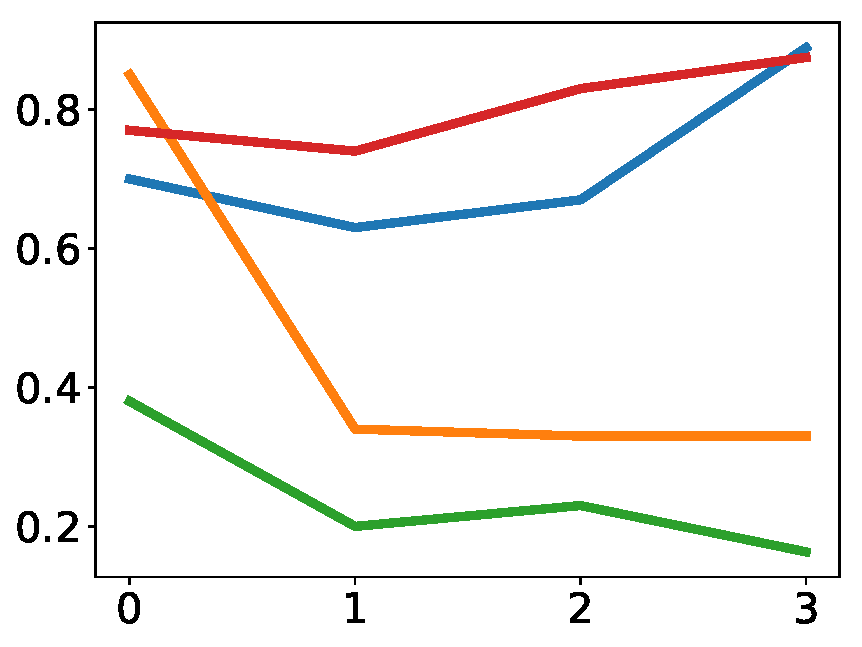
\includegraphics[width=0.24\textwidth]{figures/german-gender-m.pdf}
% 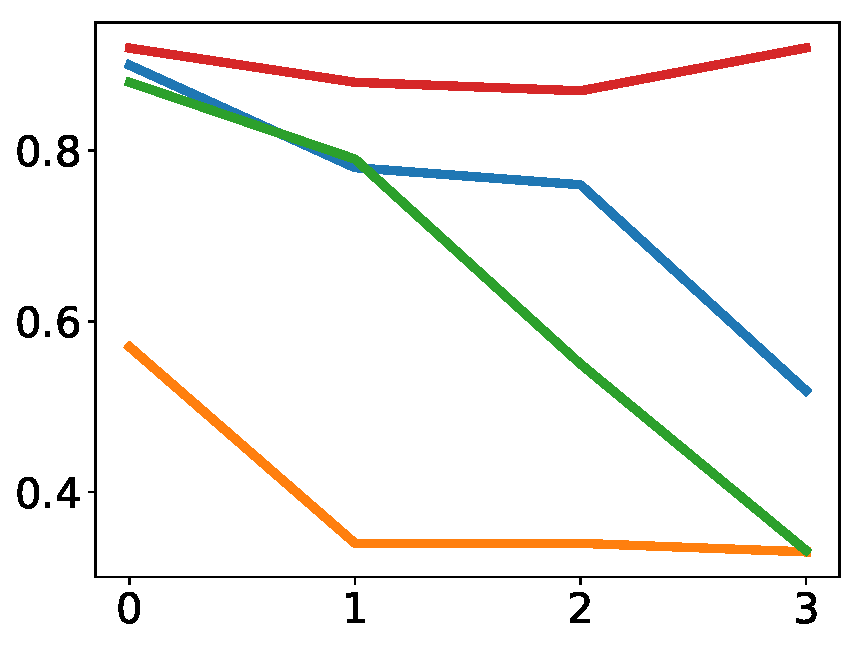
\includegraphics[width=0.24\textwidth]{figures/german-gender-f.pdf}
% 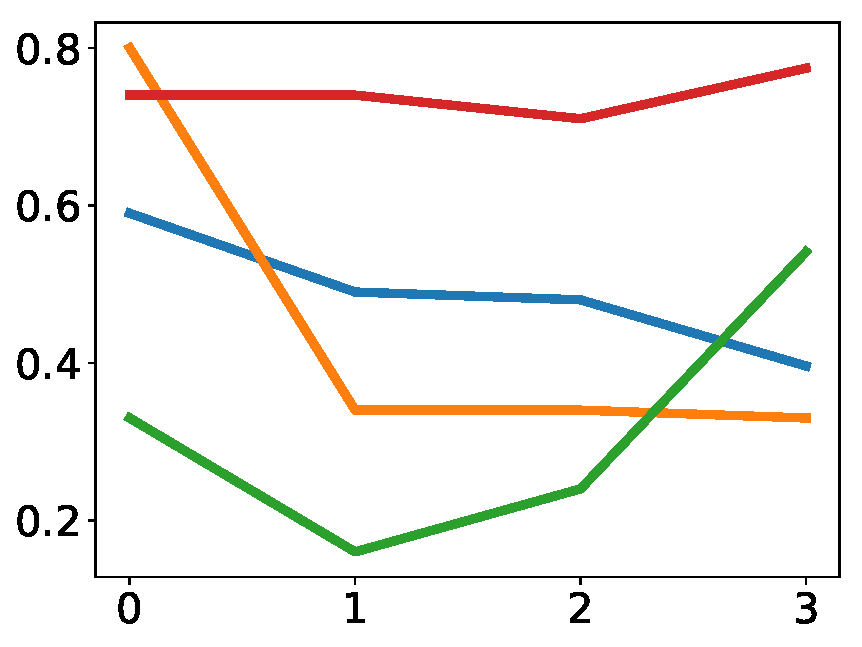
\includegraphics[width=0.24\textwidth]{figures/german-gender-n.pdf}
	\begin{tabular}{ccc}
Gender & Case & Subcategorization \\
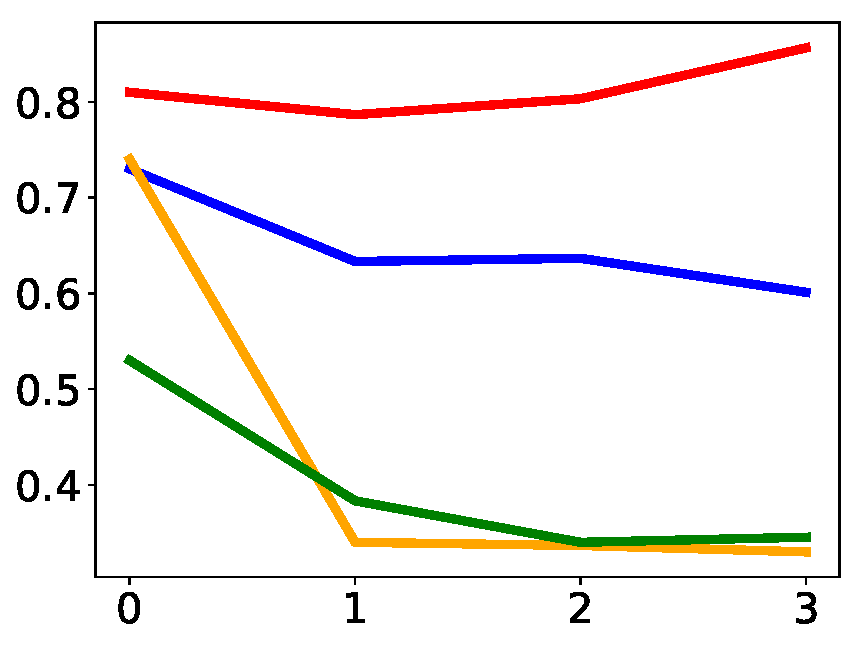
\includegraphics[width=0.28\textwidth]{figures/german-gender-total.pdf} 
		&
		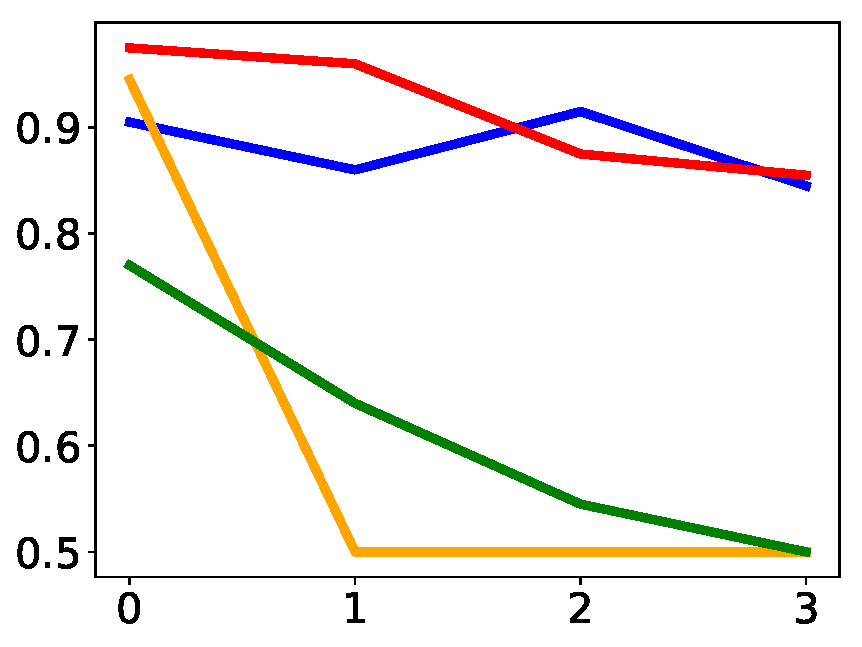
\includegraphics[width=0.28\textwidth]{figures/german-case-total.pdf}
		&
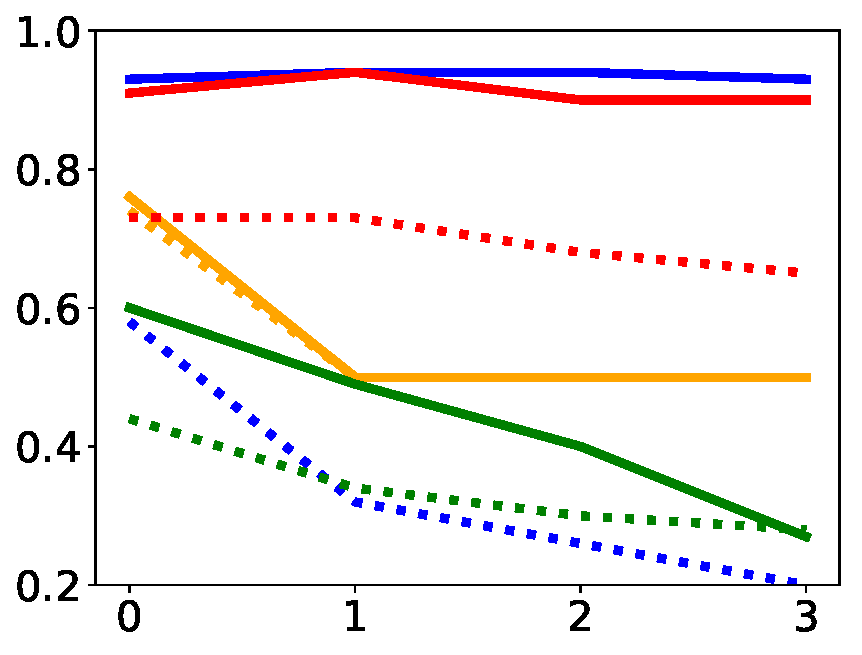
\includegraphics[width=0.28\textwidth]{figures/german-prep-with-control.pdf}
	\end{tabular}
\centering
\includegraphics[width=0.5\textwidth]{figures/german-legend.pdf}
\caption{Accuracy on the German syntax tasks, as a function of the number of intervening elements.}\label{fig:german-syntax}
\end{figure*}

% \begin{figure*}
% % 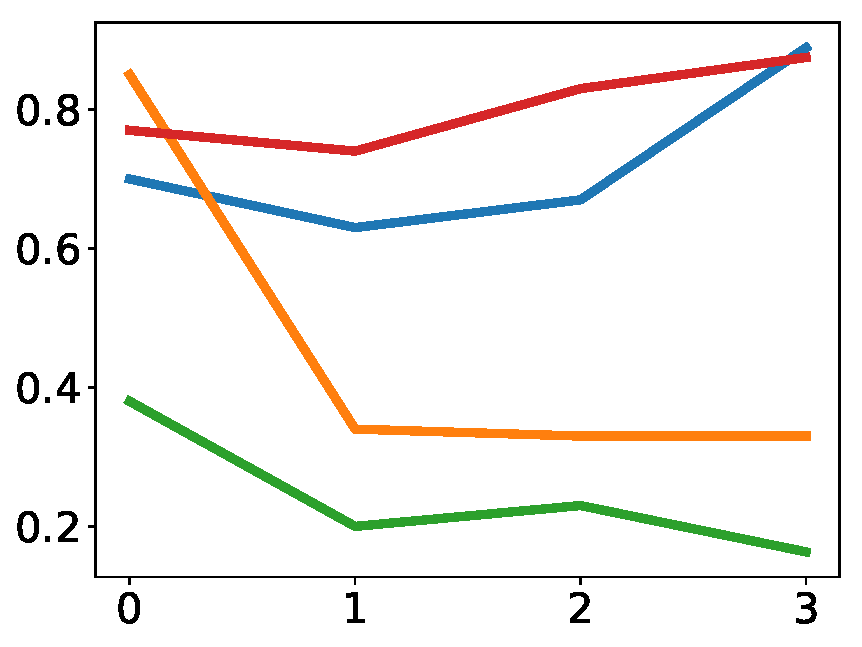
\includegraphics[width=0.24\textwidth]{figures/german-gender-m.pdf}
% % 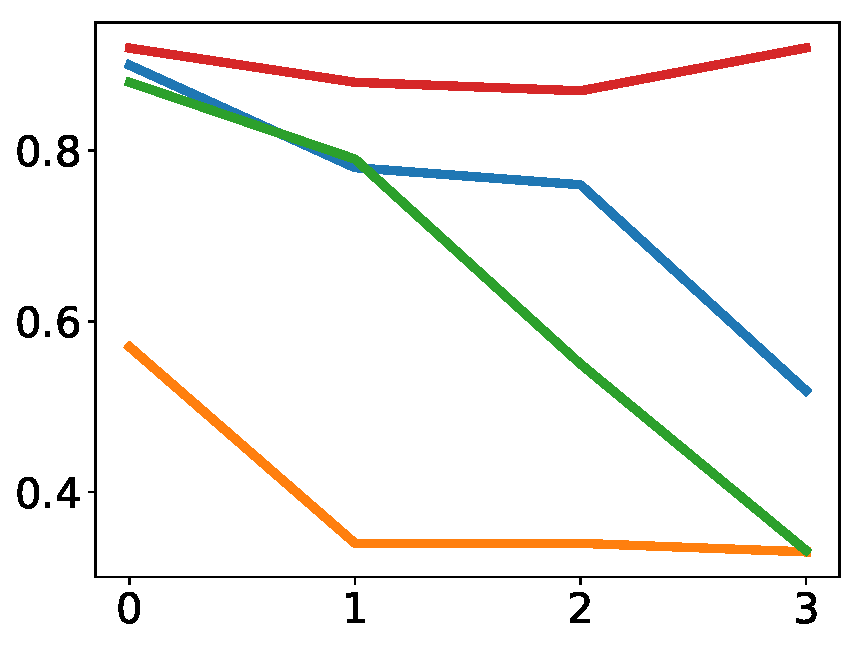
\includegraphics[width=0.24\textwidth]{figures/german-gender-f.pdf}
% % 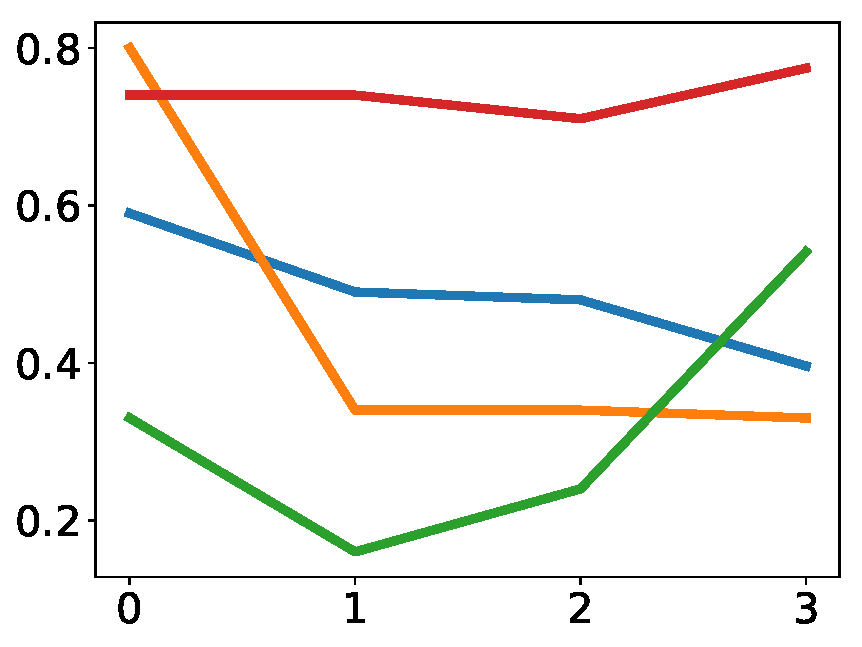
\includegraphics[width=0.24\textwidth]{figures/german-gender-n.pdf}
% 	\begin{tabular}{ccc}
% Gender & Case & Subcategorization \\
% 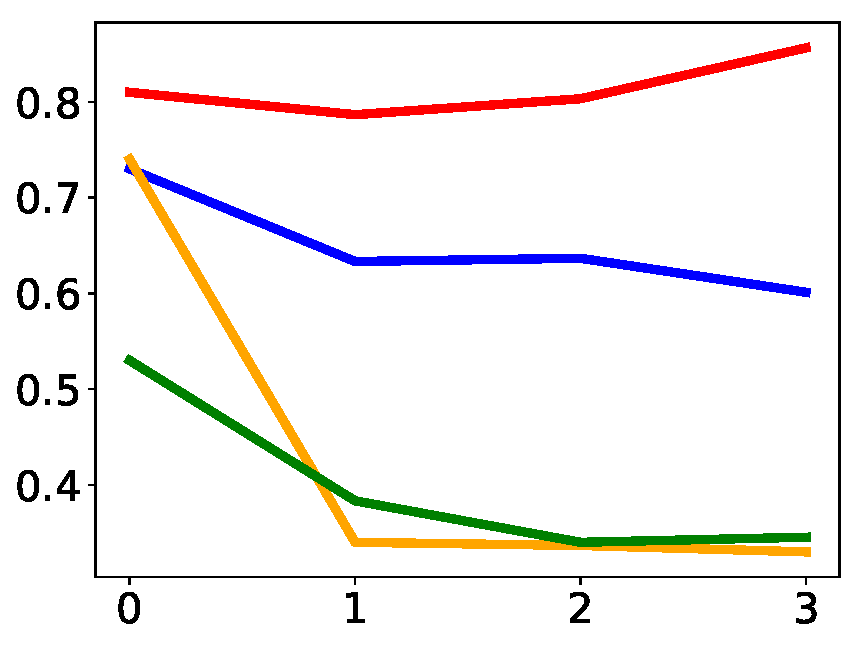
\includegraphics[width=0.33\textwidth]{figures/german-gender-total.pdf} 
% 		&
% 		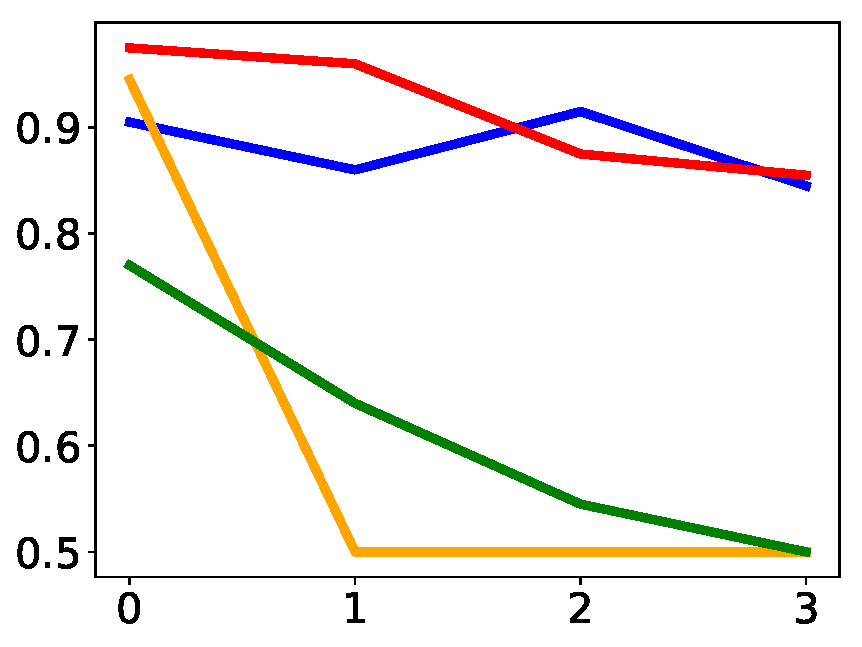
\includegraphics[width=0.33\textwidth]{figures/german-case-total.pdf}
% 		&
% 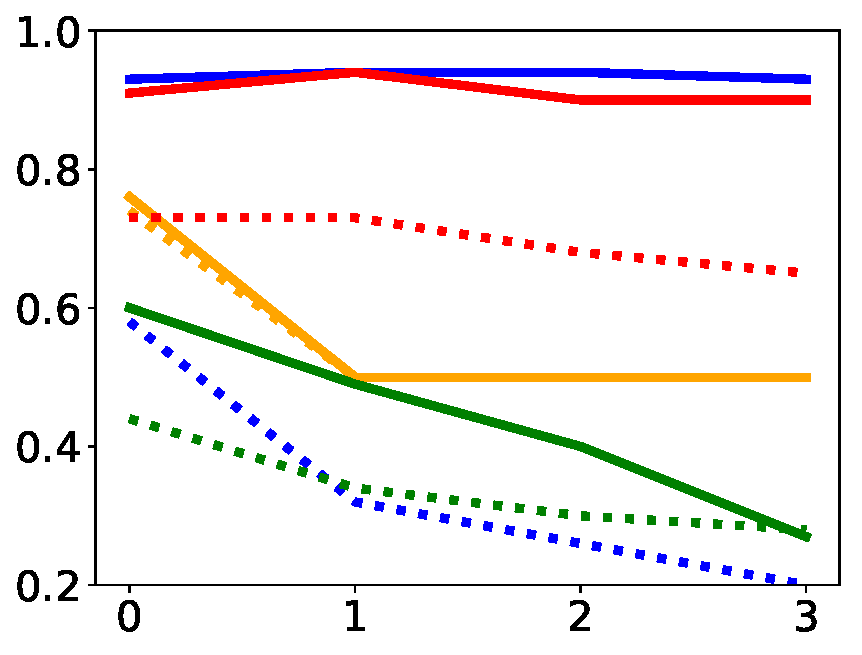
\includegraphics[width=0.33\textwidth]{figures/german-prep-with-control.pdf}
% 	\end{tabular}
% \centering
\includegraphics[width=0.5\textwidth]{figures/german-legend.pdf}
% \caption{Accuracy on the German syntax tasks, as a function of the number of intervening elements.}\label{fig:german-syntax}
% \end{figure*}


\paragraph{Case agreement}
To test the model's knowledge of case agreement between articles and
nouns, we selected the two determiners \emph{dem} and \emph{des},
which unambiguously indicate dative and genitive case, respectively,
for masculine and neuter nouns: %\textbf{Give one example.}
\ex.\ag. {\{\underline{dem}, des\}} sehr roten Baum \\
the very red {tree \emph{(dative)}} \\
\bg. {\{dem, \underline{des}\}} sehr roten Baums \\
the very red {tree \emph{(genitive)}} \\



%\begin{enumerate}[label={(\arabic*)}]
%	\item \begin{tabular}[t]{lllllll}
%	\{\underline{dem}, des\}& sehr& roten& Baum \\
%	article & adverb & adjective & noun \\
%	the & very & red & tree
%\end{tabular}
%\item \begin{tabular}[t]{lllllll}
%	\{dem, \underline{des}\}& sehr& roten& Baums \\
%	article & adverb & adjective & noun \\
%	the & very & red & tree
%\end{tabular}
%
%\end{enumerate}

We selected all noun lemmas of the
appropriate genders from the Universal Dependencies, and extracted
morphological paradigms from Wiktionary to obtain case-marked forms,
retaining only nouns unambiguously marking the two cases.  We created
four conditions, varying the amount of intervening material, as in the
gender agreement experiment (4,509 stimuli per condition).

Results are in Figure~\ref{fig:german-syntax} (center).  Again, WordNLM has
the best performance, but the LSTM CNLM is competitive as more
elements intervene. Accuracy stays well above 80\% even as three
words intervene.  The n-gram model performs well if there is no
intervening material, and at chance otherwise.  The RNN
CNLM accuracy remains above chance for one or two intervening elements, but
drops considerably.

% Considering the results for the dative and genitive separately, accuracy slightly increases in the dative case and decreases in the genitive case.
% This can be attributed to the higher baseline frequency of dative in German, suggesting that both word- and character-based networks are impacted by unigram frequencies as more words intervene.
% This effect is far more pronounced for the RNN CNLM, explaining its overall decrease to chance level.
% Again, restricting to words that are in the word-level vocabulary did not change the pattern of results.
%\begin{figure}
%% 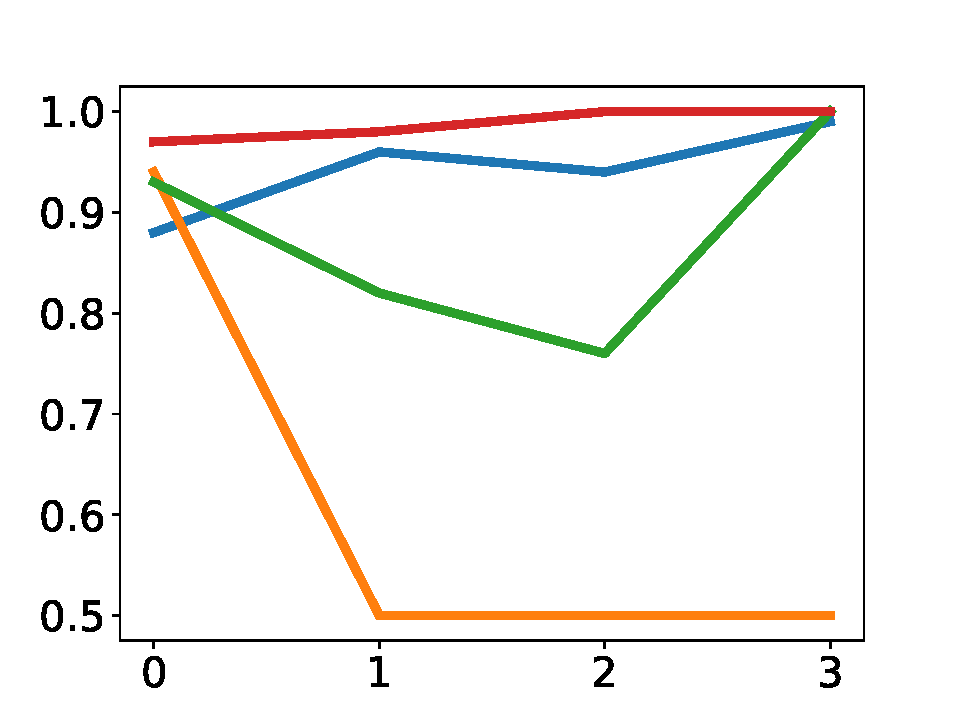
\includegraphics[width=0.23\textwidth]{figures/german-case-Dative.pdf}
%% 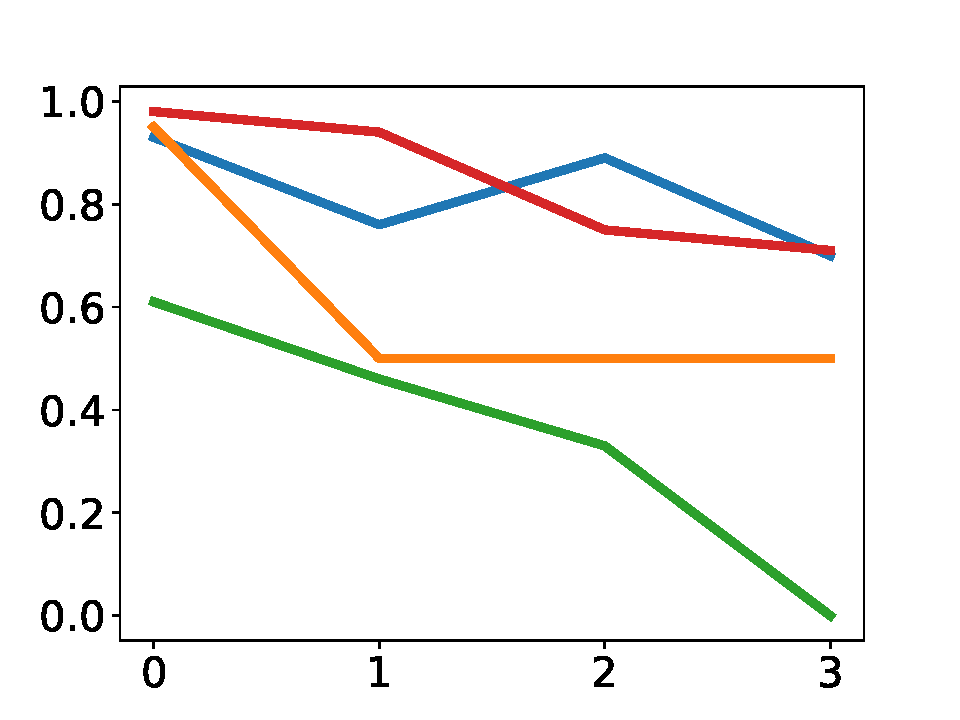
\includegraphics[width=0.23\textwidth]{figures/german-case-Genitive.pdf} \\
%
%\centering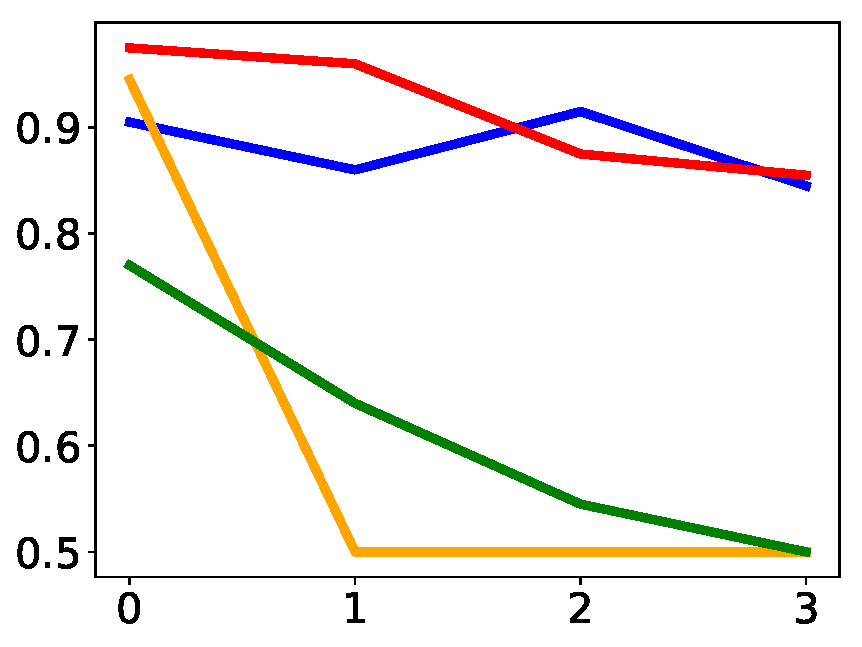
\includegraphics[width=0.24\textwidth]{figures/german-case-total.pdf}
%
%
\includegraphics[width=0.5\textwidth]{figures/german-legend.pdf}
%	\caption{\textbf{(Reduce to single figure, 2)} Accuracy on the case agreement task as a function of the number of intervening elements.}\label{fig:case}
%\end{figure}

\paragraph{Case subcategorization}
German verbs and prepositions lexically specify their object's case.  We
study the preposition \textit{mit} `with', which selects a dative
object. We use objects whose head noun is a nominalized adjective,
with regular, overtly marked case inflection.  We take all adjectives
that occur at least 100 times in the training data, excluding those
that end in -\emph{r}, as these often reflected lemmatization
problems. We then select all sentences containing a \emph{mit}
prepositional phrase in Universal Dependencies, subject to the
constraints that (1) the object is not a pronoun (replacing such items with a
nominal object often results in ungrammaticality), and (2) the object
is a continuous phrase, i.e., it is not interrupted by words that do
not belong to it. %\textbf{(please explain the latter more clearly)}.
We obtained 1,629 such sentences.  For each sentence, we remove the
prepositional phrase and replace it by a phrase of the form
\exg. mit der sehr \{rote,\ \underline{roten}\} \\
with the very red\ one \\

%\begin{enumerate}[label={(\arabic*)}]
%	\item \begin{tabular}[t]{lllllll}
%	mit & der & sehr& \{rote, \underline{roten}\} \\
%	prep & article  & adverb & adjective \\
%	with & the & very  & red one 
%\end{tabular}
%\end{enumerate}
where only the \emph{-en} (dative) version of the adjective is
compatible with the case requirement of the preposition (and the
intervening material does not disambiguate case). Note that the
correct form is longer than the wrong one. This ensures that the
probabilistic bias for shorter sequences works against the model.  We
construct three conditions by varying the presence and number of
adverbs (\emph{sehr} `very', \emph{sehr extrem} `very extremely',
\emph{sehr extrem unglaublich} `very extremely incredibly').  As a
control for baseline probabilities of the two adjectival forms, we
also created stimuli where all words up to the preposition were
removed, and computed accuracy on these stimuli.  If accuracy is lower
on these stimuli than on the full ones, we can conclude that the
baseline probabilities of the two adjective forms cannot explain
success on the task. For the n-gram count model, we only counted the
occurrences of the prepositional phrase, omitting the sentence
environment.

%\begin{figure}
%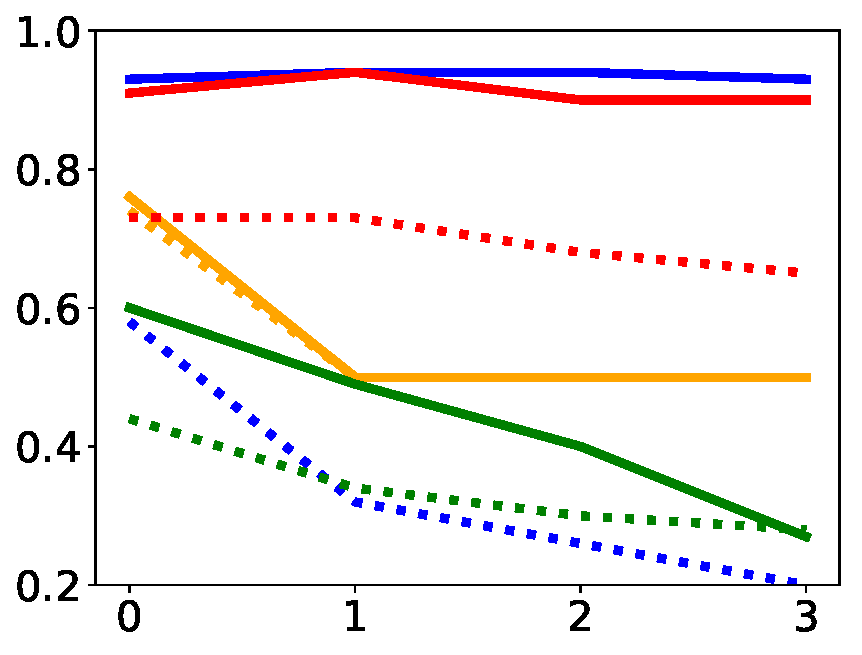
\includegraphics[width=0.48\textwidth]{figures/german-prep-with-control.pdf}
%
%
\includegraphics[width=0.48\textwidth]{figures/german-legend.pdf}
%\caption{\textbf{(Reduce to single figure, 3)} Accuracy on the subcategorization task as a function of the number of intervening elements. The dashed lines indicate accuracies on the control stimuli that do not contain the preposition.}\label{fig:prep}
%\end{figure}
%
Results are shown in Figure~\ref{fig:german-syntax} (right). Only
the n-gram model fails to outperform the control accuracy for
stimuli not including the preposition. Surprisingly, the LSTM CNLM slightly
outperforms the WordNLM, even though the CNLM is exposed
to a harder test set without OOV removal.  Neither model shows
accuracy decay as the number of adverbs increases.  As before, the
n-gram model drops to chance as adverbs intervene, while the RNN CNLM
starts with low accuracy that progressively decays below chance.

%Results are shown in Table~\ref{tab:ital-agr-results}.
%The word LSTM shows the highest overall performance, closely followed by the LSTM CNLM.
%The RNN performs well on adjective gender, and considerably worse than the CNLM on the other tasks.
%For the CNLMs, the most challenging task was article-noun gender agreement.
%Discussion case-by-case, including how we control for n-gram frequency
%and length.
%Results table with a row for each pattern and a column for each model.




\subsubsection{Italian} %\textbf{Also here, add data-set sizes.}
%\textbf{For the examples, you know the linguex packet, right?}
%\textbf{Given that you itemize by gender, can you add a baseline based
%  on picking the most frequent variant of the noun/adjective?}
% We focus on paradigms where gender and number are explicitly and
% systematically encoded and it is possible to compare same-length
% strings. We are able to extract enough stimuli that never occur in the
% training corpus, so that an n-gram control would be at chance
% level. Moreover, by experiment construction, baselines relying on
% unigram frequency are also at chance level.

\paragraph{Article-noun gender agreement}
%(1) eadj-aonoun:

Similar to German, Italian articles agree with the noun in gender;
however, Italian has a relatively extended paradigm of masculine and
feminine nouns differing only in the final vowel (-\emph{o} and
-\emph{a}, respectively), allowing us to test agreement in fully
controlled paradigms such as the following:

\ex.\ag. \{\underline{il},\ la\}  congeniale  candidato \\
the congenial candidate\ (m.) \\
\bg.  \{il,\ \underline{la}\}  congeniale  candidata \\
the congenial candidate\ (f.) \\
%\begin{enumerate}[label={(\arabic*)}]
%	\item 
%		\begin{tabular}[t]{lllllll}
%	a. & \{\underline{il}, la\} & congeniale & candidato \\
%   &  the & congenial & candidate (m.) \\
%	& \multicolumn{4}{l}{`The congenial male candidate.'} \\
%	b. & \{il, \underline{la}\} & congeniale & candidata \\
%    &the & congenial & candidate (f.) \\
%	& \multicolumn{4}{l}{`The congenial female candidate.'} \\
%\end{tabular}
%\end{enumerate}

The intervening adjective, ending in -\emph{e}, does not cue
gender. We constructed the stimuli with words appearing at least 100
times in the training corpus. We required moreover the \emph{-a}
and \emph{-o} forms of a noun to be reasonably balanced in frequency
(neither form is twice more frequent than the other), or both rather
frequent (appear at least 500 times). As the prenominal adjectives are
somewhat marked, we only considered -\emph{e} adjectives that occur
prenominally with at least 10 distinct nouns in the training corpus.
Here and below, stimuli were manually checked removing nonsensical
adjective-noun (below, adverb-adjective) combinations. Finally, adjective-noun combinations that
occurred in the training corpus were excluded, so that an n-gram
baseline would perform at chance level. We obtained 15,005 stimulus
pairs in total. % In
% addition to CNLMs and WordNLM, we tested frequency baseline choosing
% the option with the higher unigram probability (whole-stimulus corpus
% frequencies are at chance by construction).
35.8\% of them contained an adjective or noun that was
OOV for the WordNLM. Again, we report this model's results on its
full-coverage subset, where the CNLM performance is only slightly above
the one reported.

Results are shown on the first line of
Table \ref{tab:ital-agr-results}.  WordNLM shows the strongest
performance, closely followed by the LSTM CNLM.  The RNN CNLM
performs strongly above chance (50\%), but again lags behind the LSTM.

\paragraph{Article-adjective gender agreement}
We next consider agreement between articles and adjectives with an intervening adverb:
\ex.\ag. il meno \{\underline{alieno},\ aliena\} \\
the\ (m.) less alien\ one \\
\bg. la meno \{alieno,\ \underline{aliena}\} \\
the\ (f.) less alien\ one \\

%\begin{enumerate}[label={(\arabic*)}]
%	\item 
%		\begin{tabular}[t]{lllllll}
%	a. & il & meno & \{ \underline{alieno}, aliena \} \\
%   &  the (m.)& less & alien  \\
%	b. & la & meno & \{ alieno, \underline{aliena} \} \\
%    &the (f.)& less & alien one \\
%\end{tabular}
%\end{enumerate}
where we used the adverbs \emph{pi{\`u}} `more', \emph{meno} `less',
\emph{tanto} `so much'. We considered only adjectives that occurred 1K
times in the training corpus (as \emph{-a}/\emph{-o} adjectives are
very common). We excluded all cases in which the
adverb-adjective combination occurred in the training corpus, obtaining 88 stimulus pairs. Due to the restriction to common adjectives, there were no WordNLM OOVs. %
%
%Here and in the next experiment, the frequency baseline chose the version with the more common adjective.
% /checkpoint/mbaroni/char-rnn-exchange/candidate_adv_aoadj_testset.txt
Results are shown on the second line of
Table~\ref{tab:ital-agr-results}; all three models perform almost
perfectly.  Possibly, the task is made easy by the use of extremely common
adverbs and adjectives.

\begin{table}[t]
  \begin{small}
    \begin{center}
      \begin{tabular}{l|ll|c}
        & \multicolumn{2}{c|}{CNLM} & \multicolumn{1}{c}{\multirow{2}{*}{WordNLM}}\\
        &\emph{LSTM}&\emph{RNN} &  \\ \hline
% eadj-aonoun
        Noun Gender & 93.1  & 79.2 & 97.4\\
%      adv-aoadj
        Adj.~Gender & 99.5 & 98.9 & 99.5\\
% adv-aeadj
        Adj.~Number & 99.0 & 84.5 & 100.0\\
%	    & \multicolumn{4}{c|}{CNLM} & \multicolumn{2}{c|}{\multirow{2}{*}{WordNLM}}  & \multicolumn{2}{c}{\multirow{2}{*}{Frequency}}\\
%	    &\multicolumn{2}{c|}{\emph{LSTM}}&\multicolumn{2}{c|}{\emph{RNN}} & & & \\ \hline
%% eadj-aonoun
%	    Noun Gender & 96.6&89.6  & 84.4&73.9 & 99.1&95.6 & 100.0 & 0.0\\
%%      adv-aoadj
%	    Adj.~Gender & 98.9&100.0 & 100.0&97.8 & 98.9&100.0 & 55.7 & 44.3 \\
%% adv-aeadj
%	    Adj.~Number & 99.0&99.0 & 99.0&70.0 & 100.0&100.0 & 86.7 & 13.3 \\
%
      \end{tabular}
    \end{center}
  \end{small}
  \caption{\label{tab:ital-agr-results} Italian agreement results.} % For each model and test, we report percentage accuracy on two stimulus classes (masculine/feminine for gender, singular/plural for number).}
\end{table}

% \begin{table}[t]
%   \begin{small}
%     \begin{center}
%       \begin{tabular}{l|ll|l|l}
%         & \multicolumn{2}{c|}{CNLM} & \multicolumn{1}{c|}{\multirow{2}{*}{WordNLM}}  & \multicolumn{1}{c}{\multirow{2}{*}{Freq.}}\\
%         &\emph{LSTM}&\emph{RNN} &  \\ \hline
% % eadj-aonoun
%         Noun Gender & 93.1  & 79.2 & 97.4 & 50.0\\
% %      adv-aoadj
%         Adj.~Gender & 99.5 & 98.9 & 99.5 & 50.0\\
% % adv-aeadj
%         Adj.~Number & 99.0 & 84.5 & 100.0 & 50.0 \\
% %	    & \multicolumn{4}{c|}{CNLM} & \multicolumn{2}{c|}{\multirow{2}{*}{WordNLM}}  & \multicolumn{2}{c}{\multirow{2}{*}{Frequency}}\\
% %	    &\multicolumn{2}{c|}{\emph{LSTM}}&\multicolumn{2}{c|}{\emph{RNN}} & & & \\ \hline
% %% eadj-aonoun
% %	    Noun Gender & 96.6&89.6  & 84.4&73.9 & 99.1&95.6 & 100.0 & 0.0\\
% %%      adv-aoadj
% %	    Adj.~Gender & 98.9&100.0 & 100.0&97.8 & 98.9&100.0 & 55.7 & 44.3 \\
% %% adv-aeadj
% %	    Adj.~Number & 99.0&99.0 & 99.0&70.0 & 100.0&100.0 & 86.7 & 13.3 \\
% %
%       \end{tabular}
%     \end{center}
%   \end{small}
%   \caption{\label{tab:ital-agr-results} Italian agreement results.} % For each model and test, we report percentage accuracy on two stimulus classes (masculine/feminine for gender, singular/plural for number).}
% \end{table}


\paragraph{Article-adjective number agreement}
Finally, we constructed a version of the last test that probed number agreement. For feminine forms, it is possible to compare same-length phrases such as:
\ex.\ag. la meno \{\underline{aliena},\ aliene\} \\
the\ (s.) less alien\ one(s) \\
\bg. le meno \{aliena,\ \underline{aliene}\} \\
the\ (p.) less alien\ one(s) \\

%\begin{enumerate}[label={(\arabic*)}]
%	\item 
%\begin{tabular}[t]{lllllll}
%	a. & la & meno & \{ \underline{aliena}, aliene \} \\
%   &  the (s.)& less & alien one(s)  \\
%	b. & le & meno & \{ aliena, \underline{aliene} \} \\
%    &the (p.)& less & alien one(s) \\
%\end{tabular}
%\end{enumerate}
% /checkpoint/mbaroni/char-rnn-exchange/candidate_adv_aeadj_testset.txt
Stimulus selection was as in the last experiment, but we used a 500-occurrences
threshold for adjectives, as feminine plurals are less common, obtaining 99 pairs. Again, no adverb-adjective combination was attested. %  Further, we manually
There were no OOV items for the WordNLM. %
% removed adjectives that did not combine well semantically with the
% adverbs under consideration (\emph{pi{\`u}, meno, tanto}).
Results are shown on the third line of
Table~\ref{tab:ital-agr-results}; the LSTMs perform almost perfectly,
and the RNN still is strongly above chance.


